\documentclass[../main.tex]{subfiles}

\begin{document}

\section{اینترنت اشیا}

\paragraph{}
قصد داریم سیستمی برای خانه‌ی هوشمند طراحی کنیم.
در سامانه رطوبت، دما و شدت نور بر اساس سنسورهایی که در اتاق‌ها نصب شده‌اند گزارش می‌شود.
این سنسورها دارای شناسه مشخصی می‌باشند که از قبل در سخت‌افزار آن‌ها آمده است.
در کنار سنسور این سامانه تعدادی عملگر هم برای روشن کردن چراغ‌ها، جابجایی پرده و قطع-وصل شوفاژ دارد.
شما در این سیستم وظیفه‌ی طراحی پروتکل ارتباطی را دارید.

\paragraph{}
پروتکل مورد توافق تیم سخت‌افزار و نرم‌افزار \lr{JSON} می‌باشد. برای سادگی فرض کنید سنسورها داده‌ها را ارسال می‌کنند و عملگرها داده‌ها را دریافت می‌کنند.
بنابراین شما تنها نیاز به طراحی ارتباط‌های یک سویه دارید.

\paragraph{}
طرح زیر خلاصه‌ای از سامانه خانه هوشمند را نمایش می‌دهد. در نظر داشته باشید که پروتکلی که
شما طراحی می‌کنید برای ارتباط‌هایی می‌باشد که با خط‌چین مشخص شده‌اند.

\begin{figure}[h!]
  \centering
  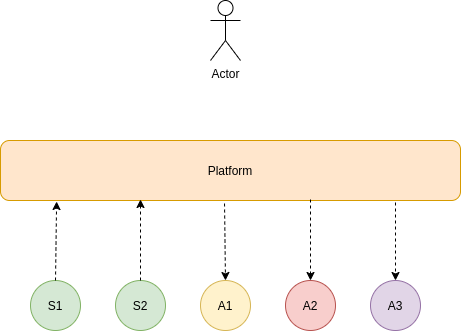
\includegraphics[scale=0.2]{json.png}
  \caption{ساختار سیستم خانه هوشمند}
\end{figure}

\paragraph{}
سنسورها همگی از یک نوع هستند و می‌توانند اطلاعات زیر را در هر بار ارسال کنند.
دقت کنید تیم سخت‌افزار طراحی را به این صورت انجام داده است که در هر بار ارسال می‌تواند همه اطلاعات را ارسال کند.
اطلاعات سنسورها به شرح زیر است:

\begin{latin}
\begin{lstlisting}
  Temperature: int / between 10 degree to 100 degree / required
  Humidity: double / between 0% to 100% / required
  Light: int / between 0 to 1024 / required
  ID: string / required
\end{lstlisting}
\end{latin}

از آنجایی که طراحی سخت‌افزار کار دشواری است پروتکل شما می‌بایست همه اطلاعات را در هر پیام ارسال کند.

\paragraph{}
عملگرها با توجه به کاری که انجام می‌دهند متفاوت هستند بنابراین اطلاعات لازم برای آن‌ها متفاوت خواهد بود.
عملگر چراغ‌ها و قطع-وصل شوفاژ به اطلاعات زیر نیاز دارد:

\begin{latin}
\begin{lstlisting}
  Status: boolean / required
  ID: string / required
\end{lstlisting}
\end{latin}

عملگر پرده به اطلاعات زیر نیاز دارد:

\begin{latin}
\begin{lstlisting}
  Height: int / between -100cm to 100cm / required
  ID: string / required
\end{lstlisting}
\end{latin}

\paragraph{}
بعد از طراحی پروتکل یک \lr{JSON Schema} نیز برای آن طراحی کنید.
این \lr{Schema} می‌بایست خصوصیات ذکر شده برای هر ارتباط را در نظر گرفته باشد.

\paragraph{}
۴ نمره


\end{document}
